\documentclass{math}

\usepackage{float}
\usepackage{graphicx}
\usepackage{subcaption}

\geometry{letterpaper, margin=0.5in}

\title{Intro to Computer Vision: HW 1}
\author{Alvin Lin}
\date{August 2017 - December 2017}

\begin{document}

\maketitle
\captionsetup{justification=centering}

\subsection*{Problem 1a}
\begin{figure}[H]
  \centering
  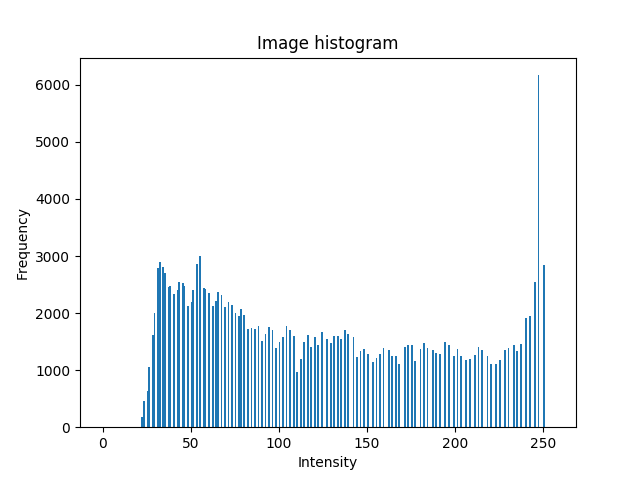
\includegraphics[width=12cm]{assets/hw_01_sonnet_histogram.png}
  \caption{Image intensity histogram for sonnet.png}
\end{figure}

\subsection*{Problem 1b}
\begin{figure}[H]
  \begin{subfigure}{0.5\linewidth}
    \centering
    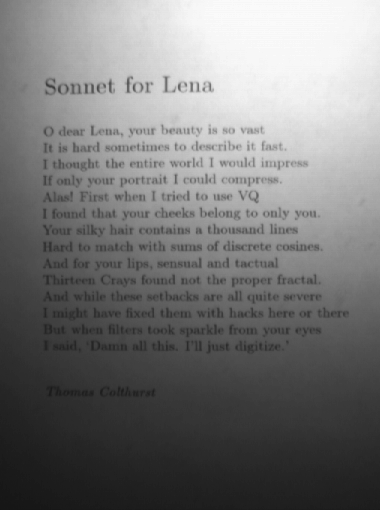
\includegraphics[width=8cm]{assets/hw_01_sonnet_original.png}
    \caption{Original image}
  \end{subfigure}
  \begin{subfigure}{0.5\linewidth}
    \centering
    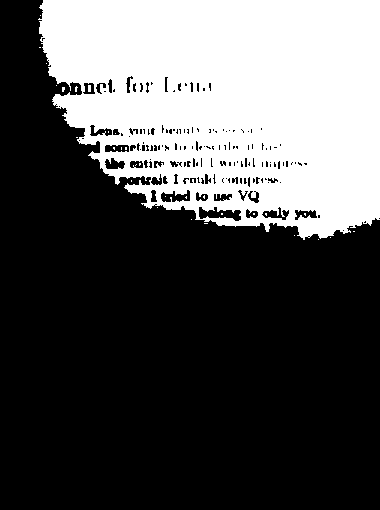
\includegraphics[width=8cm]{assets/hw_01_static_threshold.png}
    \caption{Using a static threshold of 150 intensity}
  \end{subfigure}
\end{figure}

\subsection*{Problem 1c}
\begin{figure}[H]
  \begin{subfigure}{0.33\linewidth}
    \centering
    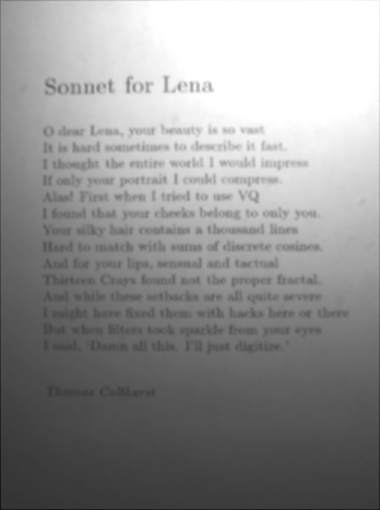
\includegraphics[width=6cm]{assets/hw_01_mean_adaptive_threshold.png}
    \caption{Mean Adaptive Threshold \\ n=1, c=30}
  \end{subfigure}
  \begin{subfigure}{0.33\linewidth}
    \centering
    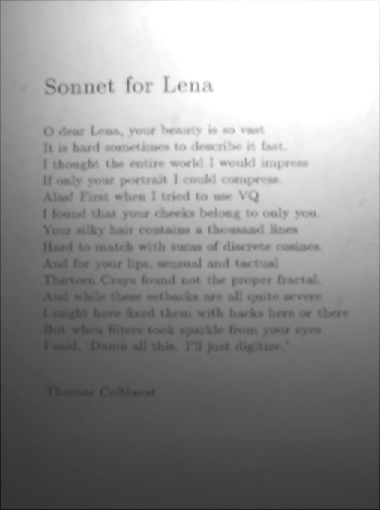
\includegraphics[width=6cm]{assets/hw_01_median_adaptive_threshold.png}
    \caption{Median Adaptive Threshold \\ n=1, c=30}
  \end{subfigure}
  \begin{subfigure}{0.33\linewidth}
    \centering
    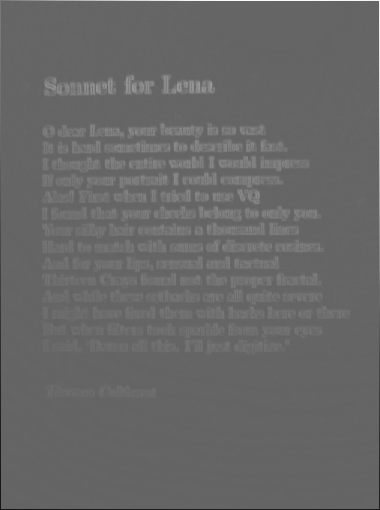
\includegraphics[width=6cm]{assets/hw_01_max_min_adaptive_threshold.png}
    \caption{Max-min Adaptive Threshold \\ n=1, c=100}
  \end{subfigure}
\end{figure}
Overall, calculating the new pixel value using the mean of its neighborhood
ended up creating more blur. Using a median method reduced the fuzziness of
the individual letters and somewhat increased contrast. Generally, the larger
the neighborhood, the more fuzzy the image became after applying the
thresholding. Therefore, only a 3x3 neighborhood centered on the pixel was used
in all of the above thresholds. Using too large of a constant \( c \) caused
the upper right of the image to whiten out the letters there, so a constant
increase of 30 was used for both the mean and median thresholds. \par
Using the max-min adaptive thresholding produced some interesting results. It
seems to have inverted the image, but did not increase the visibility of the
letters since a lot of blur was introduced to the image.

\subsection*{Problem 2a}
\begin{figure}[H]
  \begin{subfigure}{0.5\linewidth}
    \centering
    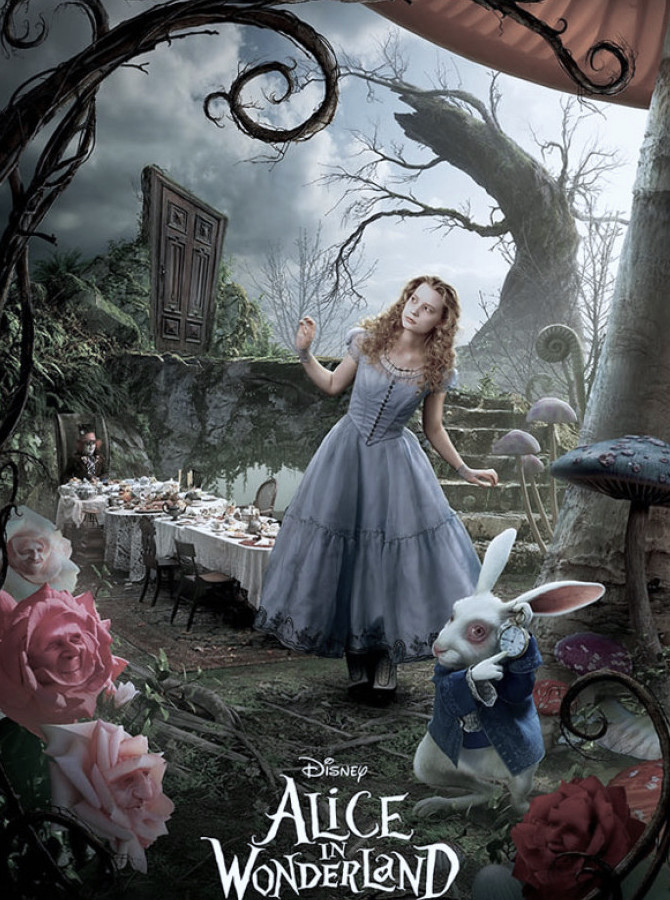
\includegraphics[width=8cm]{assets/hw_01_alice_original.png}
    \caption{Original image}
  \end{subfigure}
  \begin{subfigure}{0.5\linewidth}
    \centering
    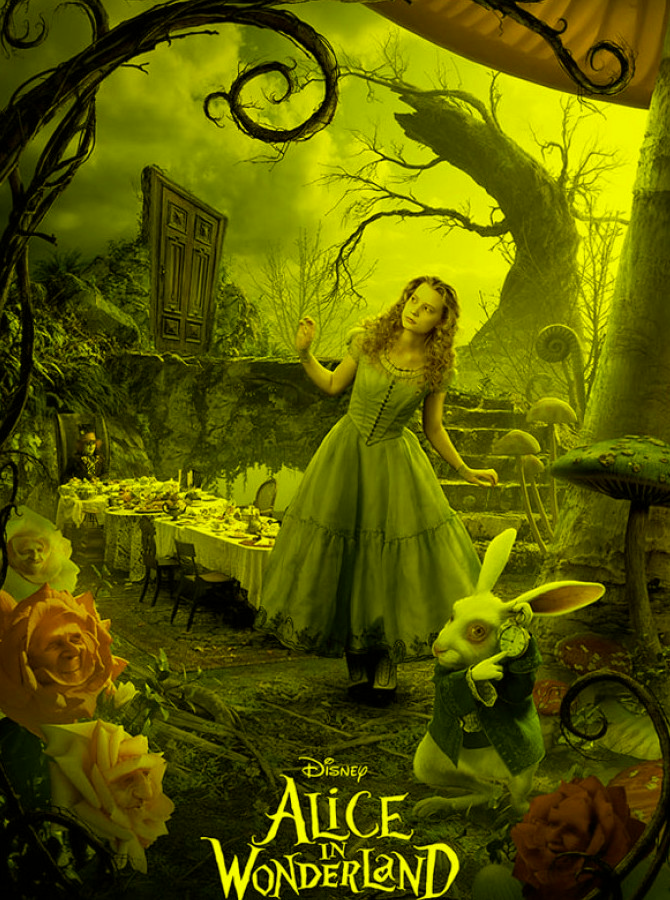
\includegraphics[width=8cm]{assets/hw_01_alice_no_blue.png}
    \caption{Alice with the blue channel set to 0}
  \end{subfigure}
\end{figure}

\subsection*{Problem 2b}
\begin{figure}[H]
  \begin{subfigure}{0.33\linewidth}
    \centering
    
\includegraphics[width=6cm]{assets/hw_01_swatch_original.png}
    \caption{Original color swatch}
  \end{subfigure}
  \begin{subfigure}{0.33\linewidth}
    \centering
    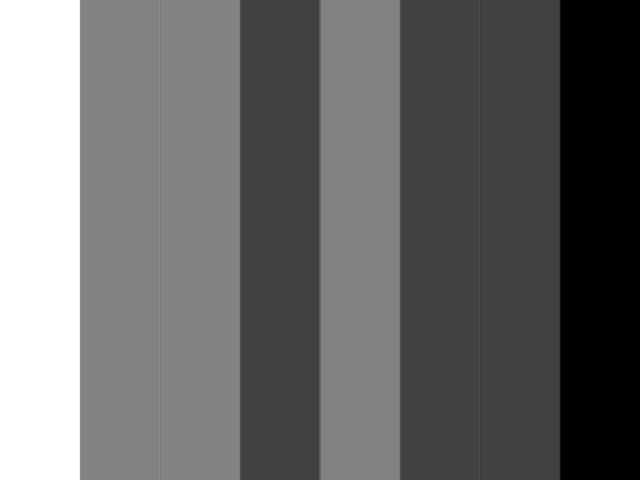
\includegraphics[width=6cm]{assets/hw_01_swatch_mean_grayscale.png}
    \caption{Intensity set to equally weighted mean of RGB}
  \end{subfigure}
  \begin{subfigure}{0.33\linewidth}
    \centering
    
\includegraphics[width=6cm]{assets/hw_01_swatch_relative_luminance.png}
    \caption{Intensity set to relative luminance}
  \end{subfigure}
\end{figure}
Using an intensity set to the weighted mean doesn't give a meaningful
difference between the colors. From the original swatch, yellow, cyan, and
magenta all look identical in their grayscale image using an equally weighted
mean. Using an intensity equal to their relatively luminance tells us that
the colors in the color swatch increase in relative luminance from right to
left.

\subsection*{Problem 2c/d}
\begin{figure}[H]
  \centering
  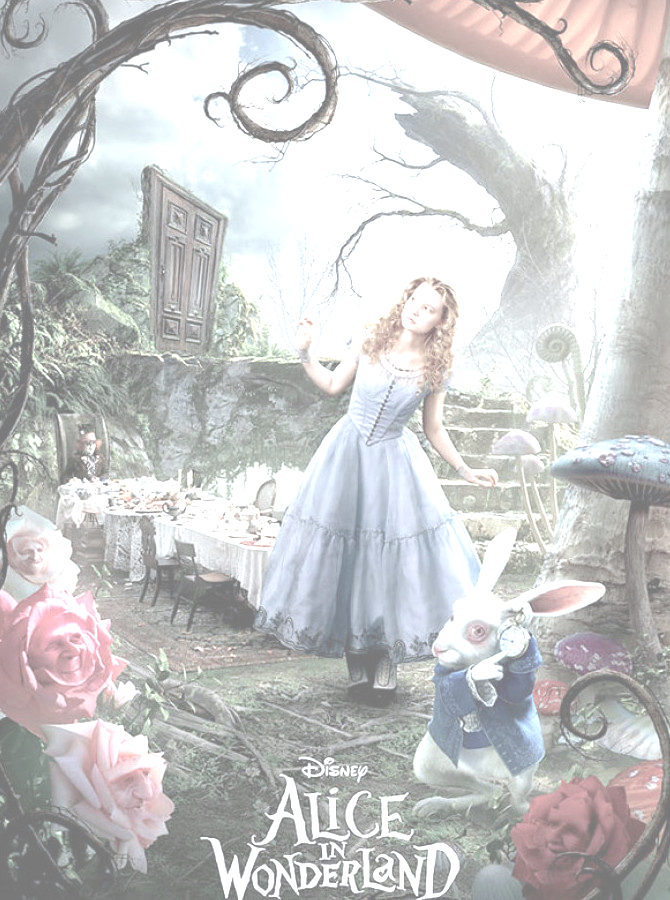
\includegraphics[width=8cm]{assets/hw_01_alice_shifted.png}
  \caption{Alice shifted by 120 in every channel and clamped}
\end{figure}
Shifting and clamping the whole image whitens the entire image. Areas in the
original image that were already light colored blend in with one another. This
causes existing dark colored regions to stand out more and reduces the variation
of intensities across the entire image. Could this be used for potential noise
reduction?

\subsection*{Problem 2e}
\begin{figure}[H]
  \centering
  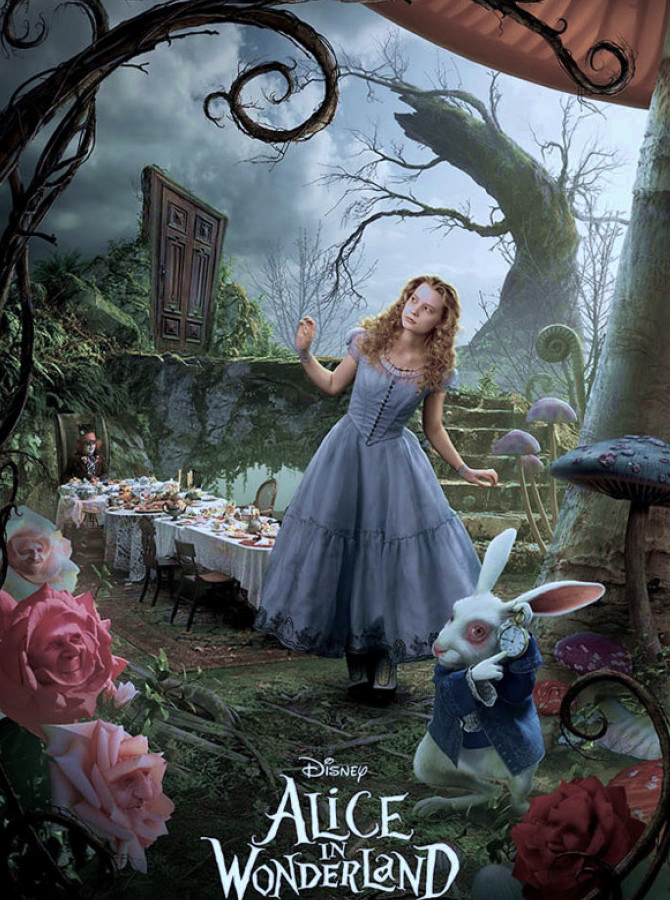
\includegraphics[width=8cm]{assets/hw_01_alice_saturated.png}
  \caption{Alice with saturation increased by 25}
\end{figure}
Increasing the saturation of the image makes the colors richer and more visible
but creates some artifacts. For example, there are now regions of blue on
Alice's forehead. Using a value of 25 seemed to be the right balance because a
lower value would have no visible effect while a higher value would increase the
amount and size of the splotches like on Alice's forehead.

\begin{center}
  If you have any questions, comments, or concerns, please contact me at
  alvin@omgimanerd.tech
\end{center}

\end{document}
